\documentclass{article}
\usepackage[T1]{fontenc}
\usepackage{amsmath, amssymb, bm, graphicx}
\usepackage{enumitem}
\usepackage{tikz}
\usepackage{tikz-3dplot}
\usepackage{pgfplots}
\pgfplotsset{compat=1.18}  % Avoid compatibility warning


\title{\textbf{Progress on Analyzing a Time Dilation Wave}}
\author{}
\date{}

\begin{document}

\maketitle

\section{Introduction}

Signal analysis is full of different methods, and I’m just trying them all to see what happens. My approach is pretty simple: shut up and compute—run the numbers first, interpret later. The key idea I’m working with is that all waves follow the same math, no matter what they represent. It’s not about whether a certain method "works" for a particular wave; it's about figuring out what the displacement actually means in physical terms.

In our original NASA NIAC proposal, we talked about using both Fourier analysis and machine learning to study signals. But instead of getting stuck on individual techniques, I realized that all these methods are connected through measure theory. So, rather than focusing on specific tools, I’m looking at the bigger picture: how measure theory acts as the common thread tying everything together.

\section{Measure Theory: The Backbone of Everything}

\subsection{The Core Ideas}

At its core, measure theory provides a rigorous foundation for analyzing functions over different kinds of spaces. It allows us to break down and analyze signals consistently. Fourier analysis itself is just a special case of measure theory, which means a lot of the other tools—such as probability, spectral methods, and even machine learning—are interconnected through this framework.

\begin{itemize}
    \item \textbf{Lebesgue Integration}: A more flexible way to define integrals compared to the usual Riemann method.
    \item \textbf{Probability and Measure Spaces}: The foundation for frequentist and Bayesian approaches.
    \item \textbf{Spectral Measures}: The bridge between Fourier analysis and more general signal decomposition methods.
\end{itemize}

\subsection{Fourier Analysis: A Short History}

In the early 19th century, Fourier was trying to understand how heat flows. His work on heat conduction led him to an unexpected discovery: even the most complicated temperature distributions could be broken down into simple, repeating patterns of sine and cosine waves. 

His method is now called a Fourier series: a way to express a function as an infinite sum of trigonometric functions:

\[
f(x) = a_0 + \sum_{n=1}^{\infty} \left( a_n \cos(n x) + b_n \sin(n x) \right).
\]

\begin{center}
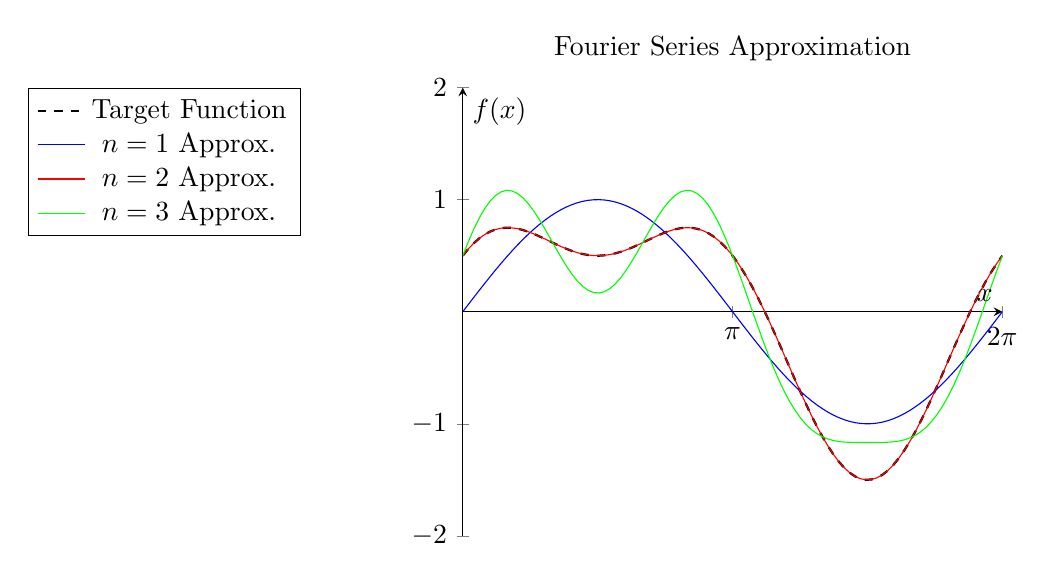
\begin{tikzpicture}
    \begin{axis}[
        domain=0:2*pi,
        samples=100,
        axis x line=middle,
        axis y line=middle,
        ymin=-2, ymax=2,
        xlabel={$x$}, ylabel={$f(x)$},
        xtick={0, 3.14, 6.28},
        xticklabels={$0$, $\pi$, $2\pi$},
        title={Fourier Series Approximation},
        legend style={at={(-0.3,1)}, anchor=north east} % Moves legend to the far left
    ]

        % Base function (target function)
        \addplot[thick, black, dashed, domain=0:2*pi] {sin(deg(x)) + cos(deg(2*x))/2};
        
        % First approximation (n=1)
        \addplot[blue, domain=0:2*pi] {sin(deg(x))};
        
        % Second approximation (n=2)
        \addplot[red, domain=0:2*pi] {sin(deg(x)) + cos(deg(2*x))/2};
        
        % Third approximation (n=3)
        \addplot[green, domain=0:2*pi] {sin(deg(x)) + cos(deg(2*x))/2 + sin(deg(3*x))/3};

        \legend{Target Function, $n=1$ Approx., $n=2$ Approx., $n=3$ Approx.}

    \end{axis}
\end{tikzpicture}
\end{center}

This equation says that no matter how messy or irregular a function might seem, it could be reconstructed entirely from smooth waves. Fourier discovered that even functions describing complex heat distributions could be rewritten in this way, making it much easier to analyze how temperature evolved over time.

But the implications of this went far beyond heat. If any function could be expressed as an infinite sum of sines and cosines, what did that mean for functions that weren’t so well-behaved? Could even jagged, discontinuous functions be decomposed into smooth waves? 

Fourier’s answer was yes. And that’s when things got weird.

\subsubsection{The Square Wave: A Function That Shouldn’t Exist}

Consider the square wave function, a simple periodic function that jumps suddenly between two values:

\[
f_{\text{square}}(x) =
\begin{cases}
    1, & -\pi < x < 0 \\
   -1, & 0 < x < \pi
\end{cases}
\]

\begin{center}
\begin{tikzpicture}
    \begin{axis}[
        domain=-2*pi:2*pi,
        samples=100,
        axis x line=middle,
        axis y line=middle,
        ymin=-1.5, ymax=1.5,
        xlabel={$x$}, ylabel={$f(x)$},
        xtick={-6.28, -3.14, 0, 3.14, 6.28},
        xticklabels={$-2\pi$, $-\pi$, $0$, $\pi$, $2\pi$},
        title={Square Wave Function}
    ]

        % Square wave segments
        \addplot[thick] coordinates {(-2*pi,-1) (-pi,-1)};
        \addplot[thick] coordinates {(-pi,1) (pi,1)};
        \addplot[thick] coordinates {(pi,-1) (2*pi,-1)};
        
        % Vertical jumps to indicate discontinuities
        \addplot[thick, dashed] coordinates {(-pi,-1) (-pi,1)};
        \addplot[thick, dashed] coordinates {(pi,1) (pi,-1)};

        % Open circles (discontinuities)
        \node at (axis cs: -pi,-1) {\textcolor{black}{$\circ$}};
        \node at (axis cs: pi,1) {\textcolor{black}{$\circ$}};

        % Filled circles (function is defined at these points)
        \filldraw[black] (axis cs: -pi,1) circle (2pt);
        \filldraw[black] (axis cs: pi,-1) circle (2pt);

    \end{axis}
\end{tikzpicture}
\end{center}

Suddenly, the comforting idea that “nice functions behave nicely” was thrown into chaos. Functions with violent, unnatural jumps were somehow being rebuilt using nothing but smooth sine waves. Even worse: those waves weren’t even behaving the way mathematicians expected. 

\begin{itemize}
    \item The right-hand side of the equation consists only of smooth sine waves.
    \item The left-hand side is a function with sharp jumps (discontinuities) at \( x = 0, \pm \pi \).
    \item Despite being an infinite sum of smooth functions, the Fourier series does not smooth out the jump.
    \item Instead, the series converges to the discontinuity but introduces oscillations, an effect now known as the Gibbs phenomenon.
\end{itemize}

This result was a major paradigm shift. It revealed that Fourier series could approximate functions far beyond the class of smooth, differentiable functions, forcing mathematicians to rethink fundamental assumptions about convergence, function representation, and the very nature of mathematical analysis.

\subsubsection{The Dirichlet Function: The Big Daddy of All Problems}

If the square function was a baby, throwing its first tantrum by introducing discontinuities, the Dirichlet function is the full-blown midlife crisis. 

The Dirichlet function is discontinuous everywhere. No pattern, no continuity, no remorse. Just pure mathematical chaos.

The function is defined as

\[
f_{\text{Dirichlet}}(x) =
\begin{cases} 
1, & x \text{ is rational} \\
0, & x \text{ is irrational}
\end{cases}
\]

and was introduced as a theoretical example rather than something meant to describe real-world phenomena. At the time, mathematicians were still grappling with what kinds of functions should be considered "legitimate" in analysis. 

From a historical perspective, the Dirichlet function was seen as an unnatural aberration. Many mathematicians, including Fourier, implicitly assumed that a function had to be reasonably well-behaved for its infinite series representation to make sense.

However, with the rise of rigorous function theory, the Dirichlet function became an essential counterexample. It forced analysts to reconsider the very nature of what a function could be. And from a Fourier series perspective, it provided a worst-case scenario: a function so fragmented that classical techniques simply collapsed.

\subsubsection{Why the Dirichlet Function Broke Fourier's Approach}

At the heart of Fourier analysis is the idea that a function can be represented as an infinite sum of sine and cosine waves:

\[
f(x) = \frac{a_0}{2} + \sum_{n=1}^{\infty} \left( a_n \cos(nx) + b_n \sin(nx) \right).
\]

where the Fourier coefficients are given by:

\[
a_n = \frac{1}{\pi} \int_{-\pi}^{\pi} f(x) \cos(n x) \,dx, \quad
b_n = \frac{1}{\pi} \int_{-\pi}^{\pi} f(x) \sin(n x) \,dx.
\]

These coefficients describe how much of each frequency contributes to the function’s reconstruction.

However, for the Dirichlet function:

\begin{itemize}
    \item It takes values 1 on rationals (a dense but countable set) and 0 on irrationals (an uncountable set).
    \item The Fourier integral sums over both rationals and irrationals.
    \item Since the rationals have measure zero in the traditional sense of Riemann integration, they contribute nothing to the integral.
    \item This results in all Fourier coefficients being zero:
\end{itemize}

\[
a_n = b_n = 0 \quad \forall n.
\]

Which means the Fourier series of the Dirichlet function is just:

\[
f_{\text{Dirichlet}}(x) = 0,
\]

which is clearly wrong. The function does exist, but it defies the assumptions Fourier’s method relies on.

\subsection{Generalizing Integration: Integrating Over Measurable Sets}

Traditional Riemann integration works by partitioning an \textbf{interval} into smaller subintervals and summing function values over them. However, this approach struggles with pathological functions, where intervals fail to provide a meaningful structure.

Lebesgue's insight was to generalize integration beyond intervals. Instead of integrating over a fixed interval, he proposed integrating over measurable sets, which are sets that can be assigned a measure equivalent to an interval.

\begin{quote}
\textbf{If a set can be mapped to an interval in a meaningful way, then we can define an integral over it.}
\end{quote}

This concept sounds simple in theory but is incredibly difficult in practice:

\begin{itemize}
    \item Finding the right measure is non-trivial. While Lebesgue measure works well in \(\mathbb{R}\), other spaces require different measures (e.g., Haar measure in group theory, probability measures in statistics).
    \item Not all sets are measurable. Some sets, like those constructed using the Axiom of Choice (e.g., the Vitali set), resist any meaningful notion of measure.
    \item Automating this process is impractical. While computers can compute Riemann integrals symbolically or numerically, determining the correct measure for a given problem often requires deep mathematical insight and domain-specific knowledge.
\end{itemize}

Thus, while Lebesgue integration vastly expands what can be integrated, it does so at the cost of requiring a much deeper understanding of the structure of the set over which the function is being integrated.

Unlike the Riemann integral, which sums function values over small partitions, the Lebesgue integral sums over values of the function itself, grouping points that share the same function value and measuring their total "size" in the domain. 

If these level sets are measurable, the function can be integrated via the Lebesgue integral:

\[
\int f \, d\mu = \int_0^\infty \mu(\{ x \mid f(x) > a \}) \, da.
\]

If these level sets are not measurable—like in the case of the Dirichlet function (which is 1 on rationals and 0 on irrationals)—then the function cannot be properly integrated in the Lebesgue sense.

Lebesgue’s generalization of integration to measurable sets fundamentally reshaped modern analysis. By removing the dependency on rigid intervals, he expanded integration to work in settings that Riemann’s approach never could, paving the way for applications in functional analysis, probability theory, and even modern physics.

\subsubsection{Why the Dirichlet Function's Integral is Zero}

With measure theory, we now recognize a crucial fact:

\begin{itemize}
    \item The set of \textbf{rational numbers} \( \mathbb{Q} \) is \textbf{countable} and therefore has \textbf{Lebesgue measure zero}.
    \item The set of \textbf{irrational numbers} \( \mathbb{R} \setminus \mathbb{Q} \) is \textbf{uncountable} and has \textbf{full measure}.
\end{itemize}

This means that, under Lebesgue integration, the contribution of the rationals to the integral is entirely insignificant: no matter how many rational numbers exist, their **total measure is still zero**.

Thus, when computing the Lebesgue integral of the Dirichlet function over any interval \( [a, b] \):

\[
\int_a^b D(x) \,dx = \int_a^b 1 \cdot \mathbb{1}_{\mathbb{Q}}(x) \,dx,
\]

where \( \mathbb{1}_{\mathbb{Q}}(x) \) is the indicator function of the rationals, we find that:

\[
\int_a^b D(x) \,dx = 0.
\]

This is because the integral assigns weight (measure) to sets, and the rationals are simply too small to contribute anything measurable.

\subsubsection{A Modern Perspective: The Energy Breakdown}

Although Fourier lacked the tools of modern function spaces and rigorous integration theory, we can understand why his approach failed using an energy-based argument.

The failure of the Dirichlet function’s Fourier series is not just a consequence of measure theory: it also manifests in how the function distributes energy among its frequency components. Even if we ignored the integral problem and attempted to construct Fourier coefficients, we would find that the energy is spread too erratically across infinitely many frequencies, making reconstruction meaningless.

The total energy of a function over \( [-\pi, \pi] \) can be thought of as the sum of its squared values (kind of like measuring how "loud" the function is overall):

\[
E(f) = \int_{-\pi}^{\pi} |f(x)|^2 \,dx.
\]

By \textbf{Parseval’s theorem}, the total energy of a function is equal to the sum of the squared Fourier coefficients:

\[
E(f) = \sum_{n=0}^{\infty} \left( \frac{a_n^2}{2} + \frac{b_n^2}{2} \right).
\]

This tells us that for Fourier reconstruction to work, the function’s energy must be properly distributed among its frequency components.

For well-behaved functions:
\begin{itemize}
    \item The Fourier coefficients decay at a controlled rate.
    \item The sum of squared coefficients converges, ensuring a proper distribution of energy.
\end{itemize}

\begin{center}
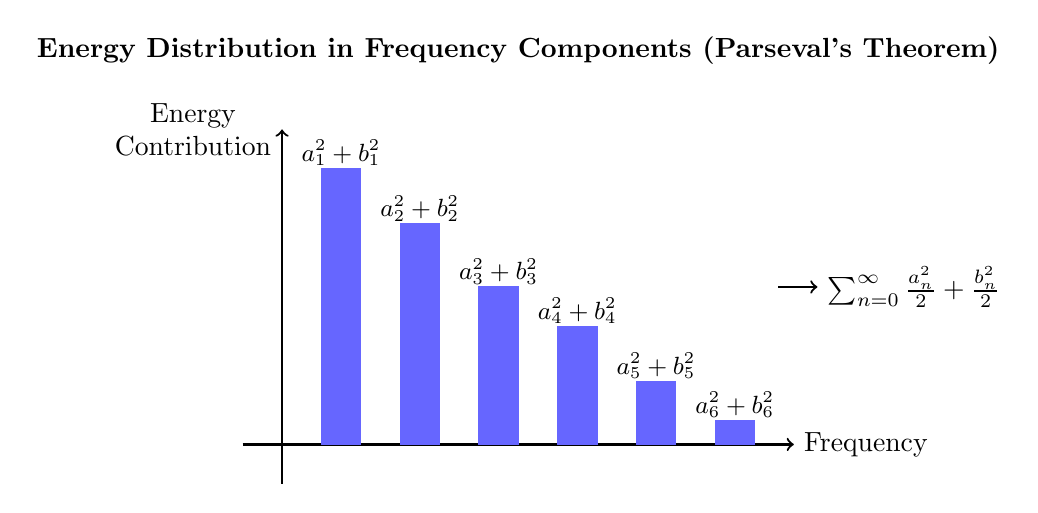
\begin{tikzpicture}
    % Axes
    \draw[thick,->] (-0.5,0) -- (6.5,0) node[right] {Frequency};
    \draw[thick,->] (0,-0.5) -- (0,4) node[left] {\parbox{2cm}{\centering Energy \\ Contribution}};

    % Bars representing squared Fourier coefficients
    \filldraw[blue!60] (0.5,3.5) rectangle (1.0,0);
    \filldraw[blue!60] (1.5,2.8) rectangle (2.0,0);
    \filldraw[blue!60] (2.5,2.0) rectangle (3.0,0);
    \filldraw[blue!60] (3.5,1.5) rectangle (4.0,0);
    \filldraw[blue!60] (4.5,0.8) rectangle (5.0,0);
    \filldraw[blue!60] (5.5,0.3) rectangle (6.0,0);

    % Labels
    \node at (0.75,3.7) {\small \( a_1^2 + b_1^2 \)};
    \node at (1.75,3.0) {\small \( a_2^2 + b_2^2 \)};
    \node at (2.75,2.2) {\small \( a_3^2 + b_3^2 \)};
    \node at (3.75,1.7) {\small \( a_4^2 + b_4^2 \)};
    \node at (4.75,1.0) {\small \( a_5^2 + b_5^2 \)};
    \node at (5.75,0.5) {\small \( a_6^2 + b_6^2 \)};

    % Sum notation
    \draw[thick, ->] (6.3,2) -- (6.8,2) node[right] {\(\sum_{n=0}^{\infty} \frac{a_n^2}{2} + \frac{b_n^2}{2}\)};
    
    % Title
    \node at (3,5.0) {\textbf{Energy Distribution in Frequency Components (Parseval's Theorem)}};

\end{tikzpicture}
\end{center}

This graph breaks down a function’s energy into its individual frequency components, and gives us a power spectrum. We do this because signals (whether they’re sound waves, electrical currents, or even stock market fluctuations) are rarely just one simple wave. Instead, they’re made up of many different frequencies combined together. The x-axis (Frequency) tells us how fast each of these components oscillates, while the y-axis (Energy Contribution) tells us how much of the total signal's energy comes from each frequency. This breakdown is useful in everything from audio processing (identifying sound patterns), to radio transmission (filtering signals), to medical imaging (reconstructing MRI scans). By understanding how a signal’s energy is spread across frequencies, we can detect patterns, remove unwanted noise, and even reconstruct missing information.

For the Dirichlet function, however:
\begin{itemize}
    \item The integral defining \( a_n \) and \( b_n \) does not behave well because of the wild oscillation between 0 and 1.
    \item The Fourier coefficients fail to decay properly, preventing meaningful reconstruction.
    \item The total energy is ill-defined in the Riemann sense, meaning the function resists being expressed as a sum of frequencies.
\end{itemize}


\begin{figure}[h]
    \centering
    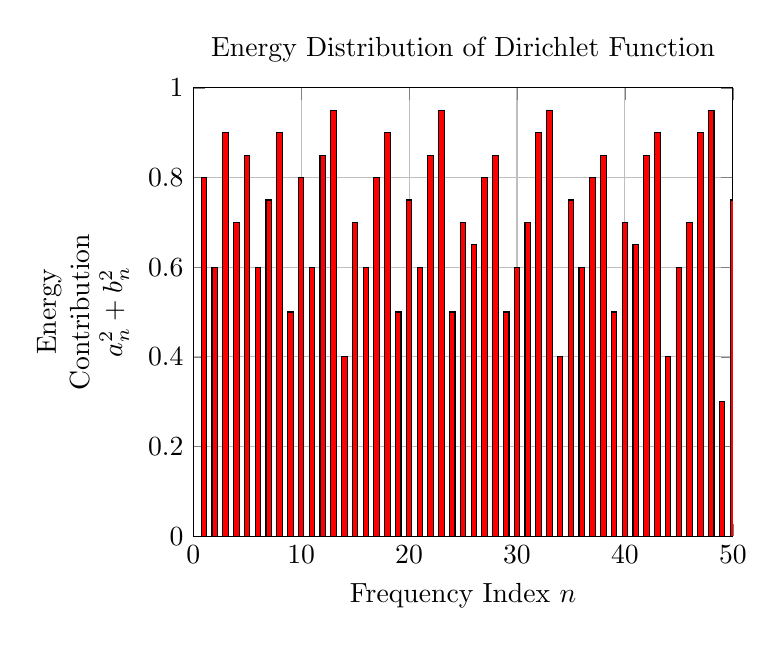
\begin{tikzpicture}
        \begin{axis}[
            title={Energy Distribution of Dirichlet Function},
            xlabel={Frequency Index \( n \)},
            ylabel={\parbox{2cm}{\centering Energy \\ Contribution \\ \( a_n^2 + b_n^2 \)}},
            xmin=0, xmax=50,
            ymin=0, ymax=1,
            xtick={0,10,20,30,40,50},
            ytick={0,0.2,0.4,0.6,0.8,1},
            grid=major,
            domain=1:50
        ]
            % Erratic energy distribution with non-decaying values as bars
            \addplot[ybar, fill=red, bar width=2pt] 
            coordinates {
                (1, 0.8) (2, 0.6) (3, 0.9) (4, 0.7) (5, 0.85) 
                (6, 0.6) (7, 0.75) (8, 0.9) (9, 0.5) (10, 0.8)
                (11, 0.6) (12, 0.85) (13, 0.95) (14, 0.4) (15, 0.7)
                (16, 0.6) (17, 0.8) (18, 0.9) (19, 0.5) (20, 0.75)
                (21, 0.6) (22, 0.85) (23, 0.95) (24, 0.5) (25, 0.7)
                (26, 0.65) (27, 0.8) (28, 0.85) (29, 0.5) (30, 0.6)
                (31, 0.7) (32, 0.9) (33, 0.95) (34, 0.4) (35, 0.75)
                (36, 0.6) (37, 0.8) (38, 0.85) (39, 0.5) (40, 0.7)
                (41, 0.65) (42, 0.85) (43, 0.9) (44, 0.4) (45, 0.6)
                (46, 0.7) (47, 0.9) (48, 0.95) (49, 0.3) (50, 0.75)
            };

        \end{axis}
    \end{tikzpicture}
    \caption{Unlike well-behaved functions, the Dirichlet function's Fourier coefficients fail to decay properly, leading to erratic energy distribution across frequencies.}
\end{figure}

This graph attempts to break down the Dirichlet function’s energy into its individual frequency components, just like a power spectrum. Normally, this would help us understand how much of a signal’s energy is stored at different frequencies. But here’s the problem: this graph is a mess.

In a well-behaved function, we expect to see the energy decay smoothly as frequency increases. This tells us that most of the energy is concentrated in the lower frequencies, making it possible to reconstruct the function efficiently. But for the Dirichlet function? No such luck. Instead of a nice, orderly drop-off, we get erratic, scattered values that don’t settle down—meaning the energy is spread unpredictably across infinitely many frequencies.

The reason the graph uses points instead of a continuous curve is that Fourier series break a function into discrete frequency components, each represented by a separate term. Normally, this would create a meaningful pattern in how energy is distributed. But here, the random-looking spikes tell us something important: there is no dominant frequency structure. The energy is chaotically spread across infinitely many frequencies, making reconstruction meaningless.

This also gives insight into why the integral of the Dirichlet function is zero. Looking at the graph, we see that the energy doesn’t accumulate in any meaningful way: it fluctuates wildly without forming a coherent structure. This reflects how the function itself oscillates erratically between 1 and 0 across its domain. Since positive and negative contributions cancel out on a large scale, the total integral over any continuous interval effectively sums to zero.

In practical applications, this kind of behavior is a nightmare. If we were trying to use this function in audio processing, it wouldn’t sound like a tone or even noise: it would be something completely incoherent. If we were using it in signal transmission, it would be utterly unusable because the signal carries no discernible structure. In short, this function fundamentally breaks the way Fourier analysis is supposed to work, which is why its decomposition is useless in any practical sense.

\section{Building Hypotheses from Measurable Structure}

Now that I finally have a physical interpretation for why displacement in time dilation happens, things are starting to click. I’m no longer just throwing mathematical tools at the problem and hoping something sticks—now I can build a structure around it. With this interpretation in place, I can define measurable sets that actually mean something in a physical context. That’s a game changer.

Here’s the key: once I know what the displacement represents physically (say, variations in gravitational potential or clock rate differences), I can start defining the sets of events, locations, or states where certain conditions hold. These sets are measurable in the Lebesgue sense, which means I can finally apply integration in a meaningful way—not just symbolically, but grounded in real-world phenomena.

\begin{itemize} \item I can now define regions of spacetime where certain thresholds of time dilation occur. \item These regions form measurable sets over which I can apply the Lebesgue integral. \item This makes it possible to compute quantities like total energy distortion, accumulated phase drift, or probabilistic bounds on signal coherence. \end{itemize}

In other words, I’m not just analyzing raw signals anymore—I’m testing physical hypotheses. This is a huge shift. Now I can ask questions like:

\begin{itemize} \item “How much cumulative distortion occurs in a region where time dilation exceeds a threshold?” \item “Is there a measurable structure to the wave that matches known physical models?” \item “Can we use these sets to train or validate machine learning models on physical data?” \end{itemize}

This shift from “shut up and compute” to “compute with a purpose” is rooted in measure theory. It gives me the ability to connect theory and observation, math and physics, intuition and calculation. With measurable sets in hand and a physical model of displacement, I can now treat signal analysis not just as a mathematical curiosity—but as a tool for uncovering real phenomena in time-dilation fields.

This is the phase where things stop being abstract and start getting real.

\section{Breaking Down the Different Methods}

To organize everything properly, I’ve categorized the methods based on their fundamental operations. There are two main dimensions: \textbf{transform-based vs. statistical methods}, and within each, whether they operate in a continuous or discrete framework.

\subsection{Transform-Based Methods (Functional \& Harmonic Analysis)}

These methods focus on converting signals into different representations, usually decomposing them into simpler components.

\subsubsection{Continuous Transform Methods}

\begin{itemize}
    \item \textbf{Fourier Analysis}: Expresses signals as sums of sinusoidal functions.
    \item \textbf{Spectral Analysis}: Uses eigenvalues and spectral decomposition to analyze frequency components.
    \item \textbf{Wavelet Transform}: A more localized frequency analysis, useful for non-stationary signals.
\end{itemize}

\subsubsection{Discrete Transform Methods}

\begin{itemize}
    \item \textbf{Discrete Fourier Transform (DFT) / Fast Fourier Transform (FFT)}: The digital version of Fourier analysis.
    \item \textbf{Z-Transform}: Used for discrete-time signals, essentially the Laplace transform for sequences.
    \item \textbf{Laplace Transform}: Used for analyzing system responses in the \(s\)-domain.
\end{itemize}

\subsection{Statistical \& Learning-Based Methods (Probability \& Data-Driven Approaches)}

These methods analyze signals by looking at statistical properties or optimizing models to learn patterns.

\subsubsection{Probabilistic \& Classical Statistics Methods}

\begin{itemize}
    \item \textbf{Frequentist Statistics}: Probability is based on observed frequencies.
    \item \textbf{Bayesian Statistics}: Uses prior and posterior distributions for inference.
    \item \textbf{Markov Models}: Models time series based on probabilistic transitions.
\end{itemize}

\subsubsection{Data-Driven \& Machine Learning Methods}

\begin{itemize}
    \item \textbf{Principal Component Analysis (PCA)}: Reduces data dimensionality by finding dominant patterns.
    \item \textbf{Support Vector Machines (SVMs)}: Classifies data using kernel methods that implicitly define measures over input spaces.
    \item \textbf{Neural Networks \& Deep Learning}: Approximate functions through layered transformations.
    \item \textbf{Empirical Risk Minimization (ERM)}: Uses probability measures over function spaces to optimize models.
\end{itemize}

\subsection{What I’ve Tried and What I’ve Seen So Far}

I’ve been applying various methods to the data and observing the results. Here’s what I’ve noticed:

\begin{itemize}
    \item \textbf{Fourier and spectral analysis} are excellent for decomposition, but they require a physical model to provide meaningful insights.
    \item \textbf{PCA and SVM} can detect patterns, but they need additional context to separate noise from actual signals.
    \item \textbf{Bayesian approaches} provide a probabilistic confidence measure in wave behavior, which is useful for modeling.
    \item \textbf{Machine learning} identifies patterns efficiently but is prone to overfitting unless the feature space is well-defined.
\end{itemize}

\section{Next Steps and What’s Coming}

Instead of committing to a single method, I am exploring \textbf{hybrid approaches}, such as combining spectral decomposition with Bayesian inference. The key insight so far is that \textbf{all waves follow the same mathematical principles}, so the challenge lies in selecting the best interpretative framework. By using measure theory as the unifying structure, I aim to ensure that no significant information is overlooked, regardless of the chosen analysis method.


\end{document}
